\section{Experiments}
\label{sec:experiment}
We conduct comprehensive experiments to answer the following research questions:

\begin{itemize}[leftmargin=1.5em]
    \item \textbf{RQ1:} How does RLCSD compare with GRPO and other OPSD baselines in terms of task performance and training stability? (\S\ref{sec:exp-main})
    \item \textbf{RQ2:} Can the proposed contrastive-hint signal improve not only RLCSD itself but also other OPSD baselines as a general-purpose component? (\S\ref{sec:exp-generality})
    \item \textbf{RQ3:} How important are the individual design choices in RLCSD, including reference-hint selection, integration with $A_{\text{ORM}}$, and the two-path loss aggregation? (\S\ref{sec:exp-ablation})
    \item \textbf{RQ4:} What broader insights does RLCSD offer for on-policy distillation (OPD)? (\S\ref{sec:exp-insights})
\end{itemize}

\subsection{Experimental Setup}
\label{sec:exp-setup}

\paragraph{Models and Datasets.} We experiment with four reasoning models, \textbf{all with thinking mode enabled during both training and validation}: Qwen3-1.7B, Qwen3-4B, Qwen3-8B~\citep{yang2025qwen3}, and Olmo-3-7B~\citep{olmo2025olmo3}. We train on two categories of tasks. (1) \textbf{Math reasoning}, for which the training data is drawn from DeepMath-103K~\citep{he2025deepmath}: we use difficulty levels 5--7 for the 1.7B model, levels 6--8 for the 4B model, and levels 7--10 for the 8B model. The test sets are AMC23~\citep{amc23}, AIME24~\citep{aime24}, and AIME25~\citep{aime25}. (2) \textbf{Logical reasoning}, for which we train on Knight-and-Knaves~\citep{xie2025logic} with 4--8 roles. The test set is also Knight-and-Knaves, comprising an in-domain test (4--8 roles, 500 questions) and an out-of-domain test (9, 10, and 11 roles, 100 questions each). Additional experiments on agentic tasks (ALFWorld~\citep{shridhar2020alfworld} and Webshop~\citep{yao2022webshop}) are provided in Appendix~\ref{app:agentic}.

\paragraph{Baselines.} We compare RLCSD against (1) \textbf{GRPO}~\citep{shao2024deepseekmath}, group relative policy optimization with binary outcome rewards verified against ground-truth answers; and the following on-policy self-distillation baselines: (2) \textbf{OPSD}~\citep{zhao2026self}, dense-logit distillation using forward KL with a per-token pointwise KL-clipping mechanism; (3) \textbf{SDPO}~\citep{hubotter2026reinforcement}, dense-logit distillation using Jensen--Shannon divergence; (4) \textbf{SRPO}~\citep{li2026unifying}, which routes successful samples to GRPO and failed samples to SDPO; and (5) \textbf{RLSD}~\citep{yang2026self}, which uses the teacher--student probability gap on sampled tokens to modulate $A_\text{ORM}$, where $A_\text{ORM}$ determines the update direction and the probability gap determines its magnitude.

\paragraph{Implementation Details.} All experiments are conducted on 8 H20 GPUs using full-parameter training. We use a learning rate of $1\times 10^{-6}$ for all tasks. For RLCSD, we keep the teacher model's weights fixed throughout training. The remaining hyperparameters are set to $K=4$, $\tau=1.3$, $\lambda=0.5$, $\delta=0.02$, and $\eta=0.5$. All prior OPSD baselines and RLCSD use dataset-provided ground-truth solutions as the correct privileged contexts. For RLCSD, negative contexts are sampled from incorrect student rollouts for the same query. All contexts include both the reasoning trace and the final answer. We use identical training and evaluation settings across methods, with maximum generation lengths of $16384$ tokens during training and $38912$ tokens during validation. Further experimental details are provided in Appendix~\ref{app:implement-detail}.

\subsection{Main Results}
\label{sec:exp-main}
% RQ1
\begin{table}[t]
\centering
\caption{Main results across model scales. Math reasoning (AMC23, AIME24, AIME25) is reported as mean@12; logical reasoning (Knight-and-Knaves) is reported as pass@1, with 4--8 Roles as the in-domain (ID) setting and 9 Roles, 10 Roles, and 11 Roles as out-of-domain (OOD) settings. \textbf{Bold} marks the best result in each block, and \underline{underline} marks the second-highest result; \textcolor{green!50!black}{green subscripts} denote the gain over the Base model.}
\label{tab:main}
\setlength{\tabcolsep}{4pt}
\resizebox{\textwidth}{!}{%
\begin{tabular}{llcccc ccccc}
\toprule
& & \multicolumn{4}{c}{\textbf{Math Reasoning} (mean@12)} & \multicolumn{5}{c}{\textbf{Logical Reasoning: Knight-and-Knaves} (pass@1)} \\
\cmidrule(lr){3-6}\cmidrule(lr){7-11}
\textbf{Model} & \textbf{Method} & AMC23 & AIME24 & AIME25 & Avg. & 4--8 Roles & 9 Roles & 10 Roles & 11 Roles & Avg. \\
\midrule

\multirow{7}{*}{Qwen3-1.7B}
 & Base  & 74.1 & 48.3 & 33.3 & 51.9 & 63.2 & 53.0 & 43.0 & 31.0 & 47.6 \\
 & GRPO  & \underline{76.6} & \underline{51.6} & \underline{37.2} & \underline{55.1} & 67.4 & \underline{59.0} & 52.0 & 34.0 & \underline{53.1} \\
 & OPSD  & 74.6 & 47.2 & 36.1 & 52.6 & 62.0 & \underline{59.0} & 51.0 & 29.0 & 50.3 \\
 & SDPO  & 73.0 & 42.2 & 31.4 & 48.9 & 63.8 & 56.0 & 52.0 & \underline{36.0} & 52.0 \\
 & SRPO  & 72.6 & 45.6 & 33.3 & 50.5 & 63.0 & \underline{59.0} & \underline{54.0} & 35.0 & 52.8 \\
 & RLSD  & 73.9 & 46.1 & 36.9 & 52.3 & \underline{68.0} & 57.0 & 49.0 & 32.0 & 51.5 \\
 \rowcolor{gray!30}
 & \textbf{RLCSD}
   & \textbf{78.2}$_{\textcolor{green!50!black}{+4.1}}$
   & \textbf{53.1}$_{\textcolor{green!50!black}{+4.8}}$
   & \textbf{38.3}$_{\textcolor{green!50!black}{+5.0}}$
   & \textbf{56.5}$_{\textcolor{green!50!black}{+4.6}}$
   & \textbf{71.8}$_{\textcolor{green!50!black}{+8.6}}$
   & \textbf{66.0}$_{\textcolor{green!50!black}{+13.0}}$
   & \textbf{61.0}$_{\textcolor{green!50!black}{+18.0}}$
   & \textbf{43.0}$_{\textcolor{green!50!black}{+12.0}}$
   & \textbf{60.5}$_{\textcolor{green!50!black}{+12.9}}$ \\

\midrule

\multirow{7}{*}{Qwen3-4B}
 & Base  & 88.6 & 72.5 & 65.3 & 75.5 & 73.2 & 67.0 & 58.0 & 42.0 & 60.1 \\
 & GRPO  & 89.1 & \underline{75.8} & 66.1 & \underline{77.0} & 75.4 & 71.0 & 61.0 & 45.0 & 63.1 \\
 & OPSD  & \underline{89.4} & 73.3 & 65.8 & 76.2 & 73.4 & 71.0 & 61.0 & 42.0 & 61.9 \\
 & SDPO  & 88.2 & 70.3 & 63.6 & 74.0 & 75.8 & 71.0 & 60.0 & 43.0 & 62.5 \\
 & SRPO  & 89.2 & 74.2 & \underline{66.7} & 76.7 & 74.6 & \textbf{76.0} & 59.0 & 47.0 & 64.2 \\
 & RLSD  & 88.9 & 72.5 & 66.1 & 75.8 & \underline{76.0} & \underline{75.0} & \underline{67.0} & \underline{49.0} & \underline{66.8} \\
 \rowcolor{gray!30}
 & \textbf{RLCSD}
   & \textbf{90.8}$_{\textcolor{green!50!black}{+2.2}}$
   & \textbf{76.4}$_{\textcolor{green!50!black}{+3.9}}$
   & \textbf{68.1}$_{\textcolor{green!50!black}{+2.8}}$
   & \textbf{78.4}$_{\textcolor{green!50!black}{+2.9}}$
   & \textbf{77.6}$_{\textcolor{green!50!black}{+4.4}}$
   & \textbf{76.0}$_{\textcolor{green!50!black}{+9.0}}$
   & \textbf{68.0}$_{\textcolor{green!50!black}{+10.0}}$
   & \textbf{51.0}$_{\textcolor{green!50!black}{+9.0}}$
   & \textbf{68.2}$_{\textcolor{green!50!black}{+8.1}}$ \\

\midrule

\multirow{7}{*}{Qwen3-8B}
 & Base  & 88.8 & 74.2 & 66.9 & 76.6 & 72.4 & 67.0 & 55.0 & 44.0 & 59.6 \\
 & GRPO  & \underline{90.1} & \underline{76.1} & \underline{69.7} & \underline{78.6} & \underline{76.8} & 75.0 & 63.0 & 49.0 & 66.0 \\
 & OPSD  & 90.0 & 74.7 & 67.2 & 77.3 & 68.8 & 65.0 & 56.0 & 46.0 & 59.0 \\
 & SDPO  & \underline{90.1} & 74.2 & 64.7 & 76.3 & 76.4 & \underline{78.0} & 66.0 & 46.0 & 66.6 \\
 & SRPO  & 89.4 & 75.6 & 65.8 & 76.9 & 76.6 & 76.0 & 63.0 & 50.0 & 66.4 \\
 & RLSD  & 89.6 & 75.6 & 67.8 & 77.7 & \underline{76.8} & \textbf{79.0} & \textbf{67.0} & \underline{52.0} & \underline{68.7} \\
 \rowcolor{gray!30}
 & \textbf{RLCSD}
   & \textbf{91.0}$_{\textcolor{green!50!black}{+2.2}}$
   & \textbf{76.4}$_{\textcolor{green!50!black}{+2.2}}$
   & \textbf{70.0}$_{\textcolor{green!50!black}{+3.1}}$
   & \textbf{79.1}$_{\textcolor{green!50!black}{+2.5}}$
   & \textbf{78.2}$_{\textcolor{green!50!black}{+5.8}}$
   & \textbf{79.0}$_{\textcolor{green!50!black}{+12.0}}$
   & \underline{66.0}$_{\textcolor{green!50!black}{+11.0}}$
   & \textbf{54.0}$_{\textcolor{green!50!black}{+10.0}}$
   & \textbf{69.3}$_{\textcolor{green!50!black}{+9.7}}$ \\

\midrule

\multirow{7}{*}{Olmo-3-7B}
 & Base  & 91.2 & 73.9 & 66.9 & 77.3 & 70.6 & 64.0 & 55.0 & 35.0 & 56.2 \\
 & GRPO  & 92.4 & \underline{75.8} & \textbf{68.9} & \underline{79.0} & \underline{73.8} & 69.0 & \underline{63.0} & 39.0 & 61.2 \\
 & OPSD  & 92.3 & 75.4 & 67.1 & 78.3 & 72.6 & \underline{70.0} & 61.0 & 39.0 & 60.7 \\
 & SDPO  & 91.8 & 74.3 & 67.2 & 77.8 & 73.4 & 68.0 & 60.0 & \underline{45.0} & \underline{61.6} \\
 & SRPO  & 91.9 & 75.2 & 65.6 & 77.6 & 73.0 & 67.0 & 62.0 & 41.0 & 60.8 \\
 & RLSD  & \underline{92.5} & 74.9 & 66.8 & 78.1 & 73.6 & 66.0 & 60.0 & 37.0 & 59.2 \\
 \rowcolor{gray!30}
 & \textbf{RLCSD}
   & \textbf{92.7}$_{\textcolor{green!50!black}{+1.5}}$
   & \textbf{76.1}$_{\textcolor{green!50!black}{+2.2}}$
   & \underline{68.6}$_{\textcolor{green!50!black}{+1.7}}$
   & \textbf{79.1}$_{\textcolor{green!50!black}{+1.8}}$
   & \textbf{75.4}$_{\textcolor{green!50!black}{+4.8}}$
   & \textbf{76.0}$_{\textcolor{green!50!black}{+12.0}}$
   & \textbf{65.0}$_{\textcolor{green!50!black}{+10.0}}$
   & \textbf{48.0}$_{\textcolor{green!50!black}{+13.0}}$
   & \textbf{66.1}$_{\textcolor{green!50!black}{+9.9}}$ \\

\bottomrule
\end{tabular}%
}
\end{table}

\begin{figure*}[t]
    \centering
    % ---------- Row 1: DeepMath ----------
    \begin{subfigure}{0.24\textwidth}
        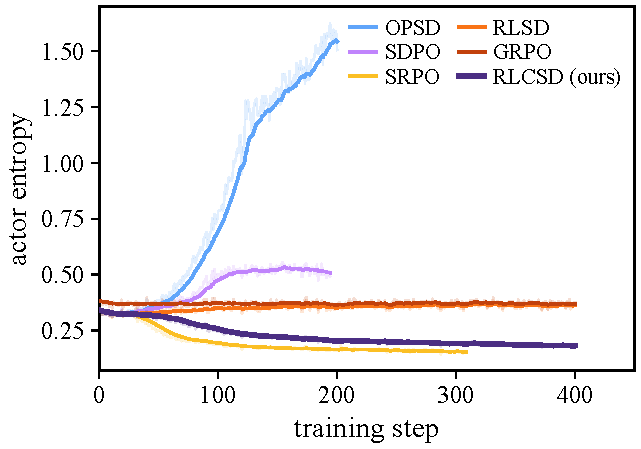
\includegraphics[width=\linewidth]{figs/curve_deepmath_entropy.pdf}
        \caption{Math: entropy}
        \label{fig:math_entropy}
    \end{subfigure}
    \hfill
    \begin{subfigure}{0.24\textwidth}
        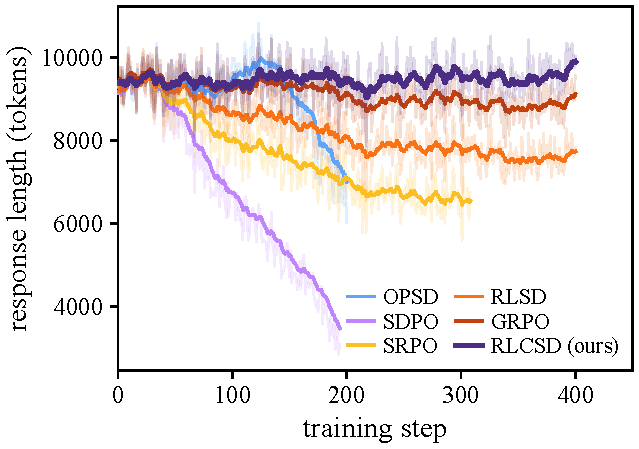
\includegraphics[width=\linewidth]{figs/curve_deepmath_length.pdf}
        \caption{Math: length}
        \label{fig:math_length}
    \end{subfigure}
    \hfill
    \begin{subfigure}{0.24\textwidth}
        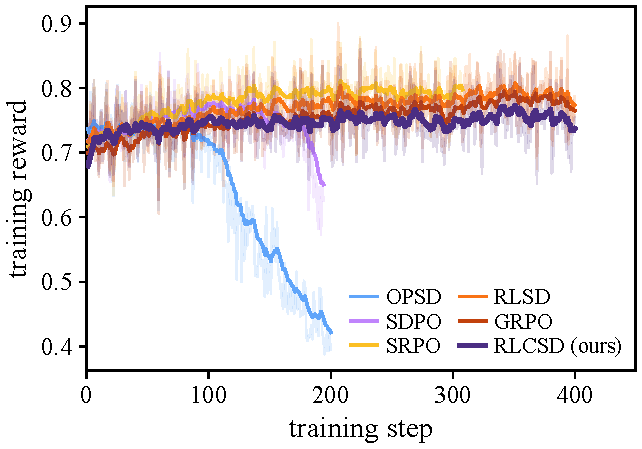
\includegraphics[width=\linewidth]{figs/curve_deepmath_reward.pdf}
        \caption{Math: reward}
        \label{fig:math_reward}
    \end{subfigure}
    \hfill
    \begin{subfigure}{0.24\textwidth}
        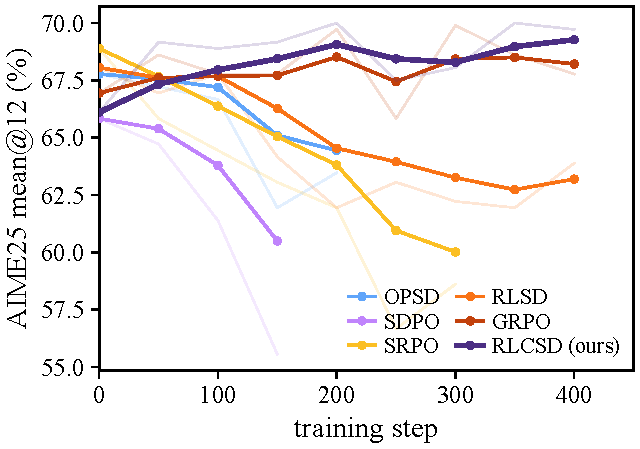
\includegraphics[width=\linewidth]{figs/curve_deepmath_val.pdf}
        \caption{Math: accuracy}
        \label{fig:math_accuracy}
    \end{subfigure}

    \vskip 0.5em

    % ---------- Row 2: Logic-KK ----------
    \begin{subfigure}{0.24\textwidth}
        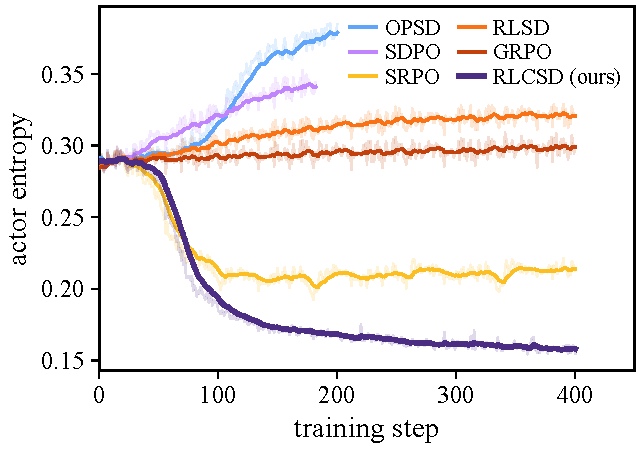
\includegraphics[width=\linewidth]{figs/curve_logic-kk_entropy.pdf}
        \caption{K\&K: entropy}
        \label{fig:KK_entropy}
    \end{subfigure}
    \hfill
    \begin{subfigure}{0.24\textwidth}
        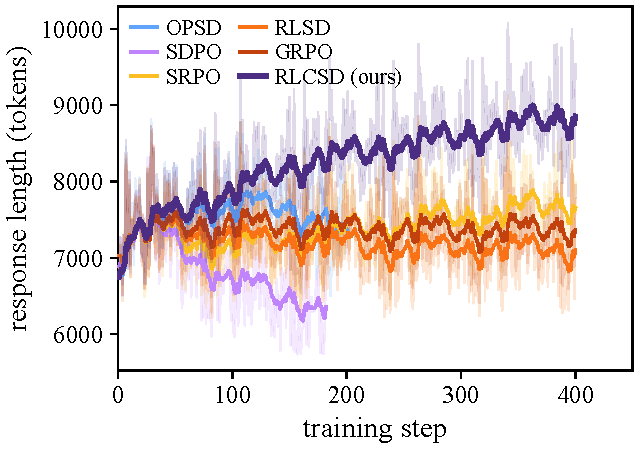
\includegraphics[width=\linewidth]{figs/curve_logic-kk_length.pdf}
        \caption{K\&K: length}
        \label{fig:KK_length}
    \end{subfigure}
    \hfill
    \begin{subfigure}{0.24\textwidth}
        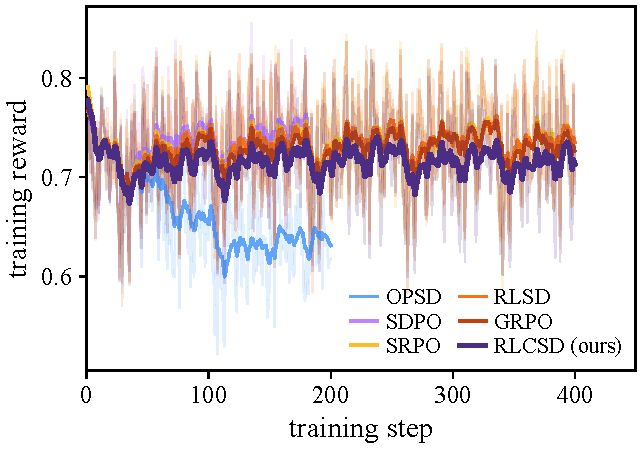
\includegraphics[width=\linewidth]{figs/curve_logic-kk_reward.pdf}
        \caption{K\&K: reward}
        \label{fig:KK_reward}
    \end{subfigure}
    \hfill
    \begin{subfigure}{0.24\textwidth}
        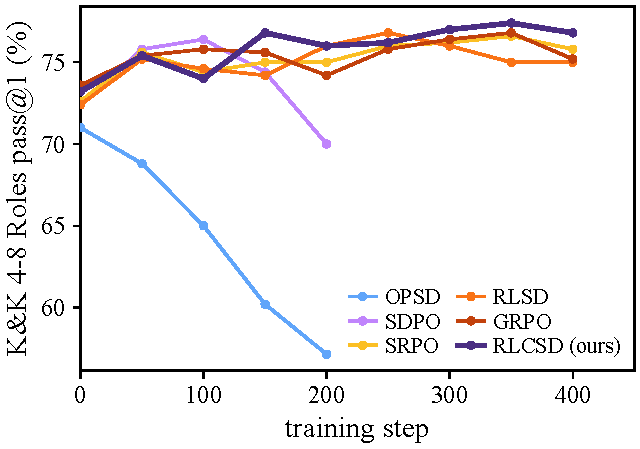
\includegraphics[width=\linewidth]{figs/curve_logic-kk_val.pdf}
        \caption{K\&K: accuracy}
        \label{fig:KK_accuracy}
    \end{subfigure}

\caption{Training dynamics of Qwen3-8B on math reasoning (top) and Knight-and-Knaves (bottom), comparing entropy, response length, training reward, and validation performance. Existing on-policy self-distillation methods exhibit premature response-length shrinkage, sometimes accompanied by rising entropy, training instability, and declining validation performance. In contrast, RLCSD maintains stable training dynamics, preserves response length on math, and gradually extends it on logical reasoning, while sustaining strong validation performance on both tasks.}
    \label{fig:training-curves}
\end{figure*}

\paragraph{Performance Comparison of RLCSD against Other Baselines.}
As shown in Table~\ref{tab:main}, RLCSD achieves the highest average performance on both math and logical reasoning across all four model scales, outperforming GRPO and prior OPSD methods. It achieves or ties the best result on nearly every individual benchmark. The average gains over the Base model are $+4.6/+12.9$ on math/logical reasoning for Qwen3-1.7B, $+2.9/+8.1$ for Qwen3-4B, $+2.5/+9.7$ for Qwen3-8B, and $+1.8/+9.9$ for Olmo-3-7B. Improvements are particularly pronounced on the harder OOD logical-reasoning settings, with gains ranging from $+9.0$ to $+18.0$ points across the 9--11 Roles benchmarks. These results suggest that the contrastive token-level signal supports generalization beyond the training distribution.

\paragraph{Failure Mode Analysis of Other On-policy Self-distillation Methods.}
Figure~\ref{fig:training-curves} shows that existing on-policy self-distillation methods exhibit \textbf{premature response-length shrinkage, sometimes accompanied by training instability}. 

\begin{itemize}
    \item On math reasoning, OPSD, SDPO, SRPO, and RLSD all show declining response lengths during training (Figure~\ref{fig:math_length}), alongside deteriorating or limited later-stage validation performance (Figure~\ref{fig:math_accuracy}). Meanwhile, OPSD and SDPO additionally exhibit rising entropy and unstable reward trajectories, showing a particularly sharp reward drop (Figures~\ref{fig:math_entropy} and~\ref{fig:math_reward}).
    \item On logical reasoning, response-length shrinkage is most evident for SDPO, while the other baselines generally plateau at shorter lengths than RLCSD (Figure~\ref{fig:KK_length}). OPSD and SDPO also exhibit increasing entropy and substantial declines in validation accuracy (Figures~\ref{fig:KK_entropy} and~\ref{fig:KK_accuracy}), with OPSD showing a sustained drop in training reward (Figure~\ref{fig:KK_reward}). 
\end{itemize}

\paragraph{Stable Dynamics of RLCSD.}
In contrast, RLCSD maintains stable training dynamics throughout optimization, keeping both policy entropy and response length stable (Figures~\ref{fig:math_entropy},~\ref{fig:math_length},~\ref{fig:KK_entropy}, and~\ref{fig:KK_length}), on par with GRPO. The key difference is that RLCSD augments GRPO's verifier-derived outcome signal with a dense token-level contrastive modulation, yielding finer-grained credit assignment without sacrificing optimization stability. As a result, RLCSD retains the same stable optimization behavior as GRPO while converging to consistently better validation performance, as shown in Figures~\ref{fig:math_accuracy} and~\ref{fig:KK_accuracy}.

\begin{table}[t]
\centering
\caption{Contrastive privileged contexts as a plug-in component. For each method, we compare a one-sided construction using a correct reference solution with a contrastive construction that additionally uses an incorrect student rollout for the same query. Math reasoning (AMC23, AIME24, AIME25) is reported as mean@12; Knight-and-Knaves is reported as pass@1, with 4--8 Roles as the in-domain (ID) setting and 9--11 Roles as out-of-domain (OOD) settings. All results use Qwen3-4B; \textbf{bold} marks the best result within each method block, including ties. $\Delta$ denotes the gain of the contrastive construction over its one-sided counterpart.}
\label{tab:contrast-generality}
\setlength{\tabcolsep}{4pt}
\resizebox{\textwidth}{!}{%
\begin{tabular}{ll cccc ccccc}
\toprule
& & \multicolumn{4}{c}{\textbf{Math Reasoning} (mean@12)} & \multicolumn{5}{c}{\textbf{Logical Reasoning: Knight-and-Knaves} (pass@1)} \\
\cmidrule(lr){3-6}\cmidrule(lr){7-11}
\textbf{Method} & \textbf{Context construction} & AMC23 & AIME24 & AIME25 & Avg. & 4--8 Roles & 9 Roles & 10 Roles & 11 Roles & Avg. \\
\midrule
\multirow{3}{*}{OPSD}
  & One-sided & 89.4 & 73.3 & 65.8 & 76.2 & 73.4 & \textbf{71.0} & \textbf{61.0} & 42.0 & 61.9 \\
  & Contrastive & \textbf{89.6} & \textbf{75.6} & \textbf{66.4} & \textbf{77.2} & \textbf{74.2} & \textbf{71.0} & \textbf{61.0} & \textbf{45.0} & \textbf{62.8} \\
\cmidrule(lr){2-11}
  & $\Delta$ & \up{+0.2} & \up{+2.3} & \up{+0.6} & \up{+1.0} & \up{+0.8} & \noup{0.0} & \noup{0.0} & \up{+3.0} & \up{+0.9} \\
\midrule
\multirow{3}{*}{RLSD}
  & One-sided & 88.9 & 72.5 & 66.1 & 75.8 & 76.0 & \textbf{75.0} & \textbf{67.0} & \textbf{49.0} & 66.8 \\
  & Contrastive & \textbf{89.8} & \textbf{75.3} & \textbf{66.4} & \textbf{77.2} & \textbf{76.4} & \textbf{75.0} & \textbf{67.0} & \textbf{49.0} & \textbf{66.9} \\
\cmidrule(lr){2-11}
  & $\Delta$ & \up{+0.9} & \up{+2.8} & \up{+0.3} & \up{+1.4} & \up{+0.4} & \noup{0.0} & \noup{0.0} & \noup{0.0} & \up{+0.1} \\
\midrule
\multirow{3}{*}{RLCSD}
  & One-sided & 88.9 & 73.1 & 62.5 & 74.8 & 73.8 & 71.0 & 58.0 & 43.0 & 61.5 \\
  & Contrastive & \textbf{90.8} & \textbf{76.4} & \textbf{68.1} & \textbf{78.4} & \textbf{77.6} & \textbf{76.0} & \textbf{68.0} & \textbf{51.0} & \textbf{68.2} \\
\cmidrule(lr){2-11}
  & $\Delta$ & \up{+1.9} & \up{+3.3} & \up{+5.6} & \up{+3.6} & \up{+3.8} & \up{+5.0} & \up{+10.0} & \up{+8.0} & \up{+6.7} \\
\bottomrule
\end{tabular}%
}
\end{table}


\begin{figure}[t]
  \centering
  % ===== 左侧大图：OPSD =====
  \begin{minipage}[t]{0.49\textwidth}
    \centering
    % 本浮动体里第一个 subfigure 会把 figure 计数器 7->8，借此作为本图号
    \begin{subfigure}[t]{0.49\linewidth}
      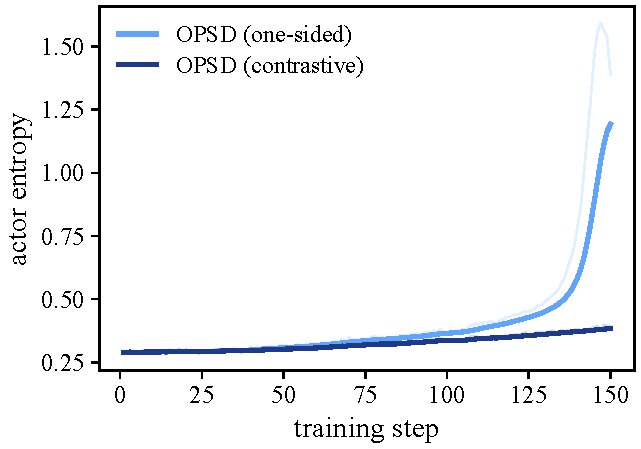
\includegraphics[width=\linewidth]{figs/ectr_logic_opsd_entropy.pdf}
      \caption{Entropy}
      \label{fig:opsd-entropy}
    \end{subfigure}
    \hfill
    \begin{subfigure}[t]{0.49\linewidth}
      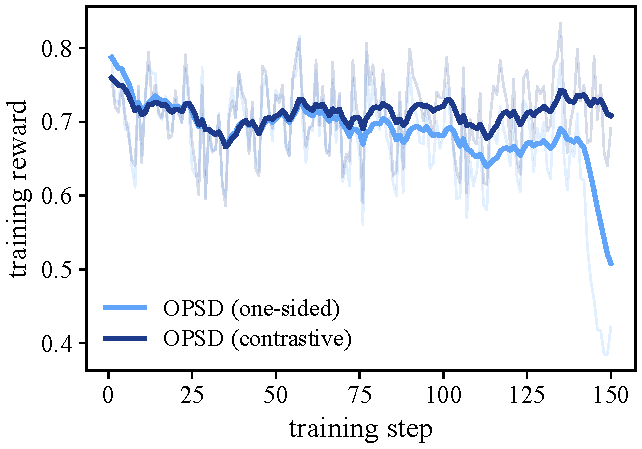
\includegraphics[width=\linewidth]{figs/ectr_logic_opsd_reward.pdf}
      \caption{Training reward}
      \label{fig:opsd-reward}
    \end{subfigure}
    \addtocounter{figure}{-1}% 抵消下面 \captionof 的多余 +1，复用图号 8
    \captionof{figure}{Effect of the contrast mechanism on OPSD for the K\&K task (Qwen3-4B).  Without contrast, the actor entropy explodes and training
      destabilizes; adding contrast keeps the entropy bounded~(a) and yields a
      stable training reward~(b).}
    \label{fig:contrast_opsd}
  \end{minipage}
  \hfill
  % ===== 右侧大图：response length =====
  \begin{minipage}[t]{0.49\textwidth}
    \centering
    \stepcounter{figure}% 此时子图不再自动 +1，需手动把图号推进到 9
    \setcounter{subfigure}{0}% 右图子标号重新从 (a) 开始
    \begin{subfigure}[t]{0.49\linewidth}
      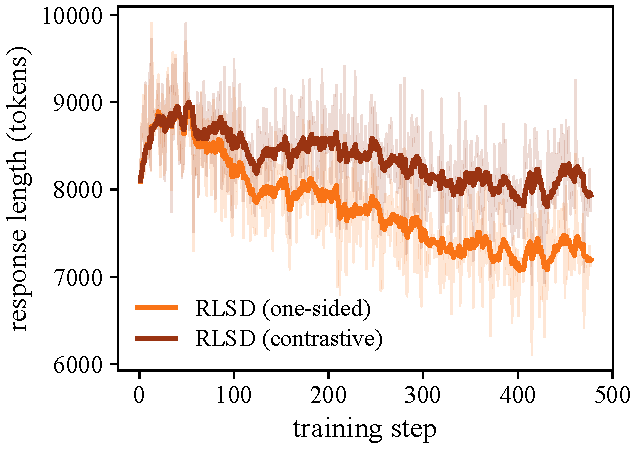
\includegraphics[width=\linewidth]{figs/ectr_math_rlsd_length.pdf}
      \caption{RLSD}
      \label{fig:rlsd-len}
    \end{subfigure}
    \hfill
    \begin{subfigure}[t]{0.49\linewidth}
      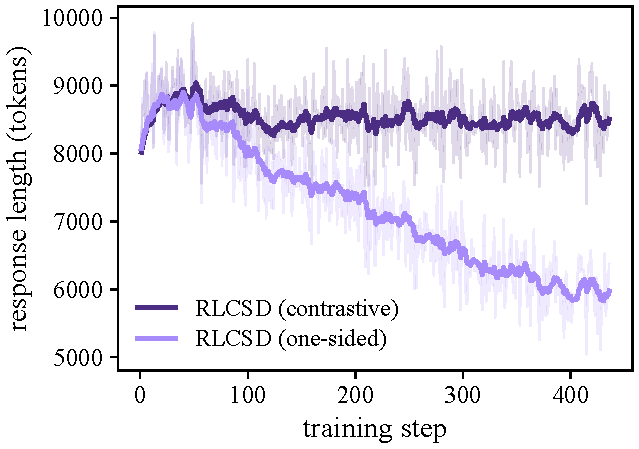
\includegraphics[width=\linewidth]{figs/ectr_math_rlcsd_length.pdf}
      \caption{RLCSD}
      \label{fig:rlcsd-len}
    \end{subfigure}
    \addtocounter{figure}{-1}% 复用图号 9
    \captionof{figure}{Effect of the contrast mechanism on response length for
      math tasks (Qwen3-4B). contrast mitigates premature response-length shrinkage for both RLSD~(a) and
      one-sided RLCSD ablation~(b), preserving longer reasoning traces that benefit late-stage
      training.}
    \label{fig:contrast_length}
  \end{minipage}
\end{figure}

\subsection{Contrastive Privileged Contexts as a General-Purpose Component}
\label{sec:exp-generality}

A central claim of this work is that the contrastive construction is not specific to RLCSD, but serves as a general principle for purifying privileged token-level signals. To test this claim, we apply it to two representative on-policy self-distillation methods from different families: OPSD~\citep{zhao2026self}, a dense full-distribution distillation method, and RLSD~\citep{yang2026self}, an advantage-modulation method. For each method, we keep the underlying optimization unchanged and compare two privileged-context constructions: \textbf{(1) one-sided}, which uses the dataset-provided ground-truth reasoning trace as the positive context; and \textbf{(2) contrastive}, which contrasts the signal induced by this positive context with that induced by an incorrect hint sampled from student rollouts for the same query.

\paragraph{How the contrast enters each method.}
The two method families incorporate the contrast differently. For advantage-modulation methods (RLSD and RLCSD), the contrast acts at the scalar level: the per-token signal
\[
e_{\mathrm{ctr},t} = \log \pi_T(y_t\mid x, y_c^*, y_{<t}) - \log \frac{1}{K}\sum_k \pi_T(y_t\mid x, y_{w,k}^*, y_{<t})
\]
replaces the one-sided $e_{c,t}$ as the modulation of $A_{\mathrm{ORM}}$. OPSD, by contrast, incorporates the signal at the \emph{distribution} level. Following a classifier-free-guidance formulation~\citep{ho2022classifier}, we replace the OPSD target $\pi_T(\cdot\mid x, y_c^*, y_{<t})$ with a contrastively amplified target:
\begin{equation}
q_{\text{target}} = \mathrm{softmax}\big((1+\alpha)\,\ell_c - \alpha\,\ell_w\big),
\end{equation}
where $\ell_c$ and $\ell_w$ are the teacher logits under the correct and incorrect hints, respectively, and $\alpha\ge 0$ controls the guidance strength ($\alpha=0$ recovers vanilla OPSD). The per-token loss is further gated by a soft mask
\begin{equation}
w_t \;=\; \frac{D_t}{D_t + \tau}, \qquad D_t \;=\; \mathrm{KL}\!\left(\pi_T(\cdot\mid x, y_w^*, y_{<t})\,\big\|\,\pi_T(\cdot\mid x, y_c^*, y_{<t})\right),
\end{equation}
with $\tau\!\ge\!0$ ($\tau\!=\!0$ disables the mask), and the final objective is $\sum_t w_t\,\mathrm{KL}(q_{\text{target},t}\,\|\,\pi_{\theta}(\cdot\mid x, y_{<t}))$.

\paragraph{Results.}

\textbf{(1) The contrastive signal improves performance across different methods.} As shown in Table~\ref{tab:contrast-generality}, the contrastive construction consistently improves the math and K\&K averages across all three methods. For OPSD, it yields gains of $1.0$ and $0.9$ points on math and K\&K, respectively. For RLSD, it improves the math average by $1.4$ points, including a $2.8$-point gain on AIME24, with a marginal gain of $0.1$ points on K\&K. RLCSD shows the largest improvements, gaining $3.6$ points on math and $6.7$ points on K\&K over its one-sided counterpart. Together, these results demonstrate that the contrastive construction benefits multiple methods, supporting its applicability as a plug-in component beyond RLCSD.

\textbf{(2) The contrastive signal mitigates premature response-length shrinkage and training instability.} On K\&K, adding contrast to OPSD curbs entropy growth and stabilizes training reward (Figure~\ref{fig:contrast_opsd}). On math, it mitigates premature response-length shrinkage in RLSD (Figure~\ref{fig:rlsd-len}) and RLCSD (Figure~\ref{fig:rlcsd-len}), whose one-sided ablation exhibits a pronounced decline in response length. These observations are consistent with the failure patterns identified in Section~\ref{sec:exp-main} and suggest that contrasting correct and incorrect privileged contexts helps preserve useful token-level supervision across different optimization formulations.

\subsection{Ablation of Key Design Choices}
\label{sec:exp-ablation}

\begin{table}[t]
\centering
\caption{Ablation of key design choices in RLCSD (Qwen3-4B). Each variant removes a single component from the full method. Math reasoning (AMC23, AIME24, AIME25) is reported as mean@12; Knight-and-Knaves (pass@1) uses roles 4--8 as in-domain (ID) and roles 9/10/11 as out-of-domain (OOD). Bold marks the best result in each column.}
\label{tab:ablation}
\small
\resizebox{\textwidth}{!}{%
\begin{tabular}{lccccccccc}
\toprule
& \multicolumn{4}{c}{Math Reasoning (mean@12)} & \multicolumn{5}{c}{Logical Reasoning: Knight-and-Knaves (pass@1)} \\
\cmidrule(lr){2-5} \cmidrule(lr){6-10}
Method & AMC23 & AIME24 & AIME25 & Avg. & 4--8 Roles & 9 Roles & 10 Roles & 11 Roles & Avg. \\
\midrule
RLCSD (full) & \textbf{90.8} & \textbf{76.4} & \textbf{68.1} & \textbf{78.4} & \textbf{77.6} & \textbf{76.0} & \textbf{68.0} & \textbf{51.0} & \textbf{68.2} \\
$-$ $K$-marginal negative hint & 89.3 & 73.2 & 67.8 & 76.8 & 76.4 & 71.0 & 63.0 & 47.0 & 64.4 \\
$+$ target rollout in hint pool & 89.1 & 73.4 & 68.0 & 76.8 & 75.8 & 70.0 & 63.0 & 46.0 & 63.7 \\
$-$ $A_{\mathrm{ORM}}$ anchoring & 88.6 & 72.1 & 66.3 & 75.7 & 74.6 & 69.0 & 61.0 & 45.0 & 62.4 \\
$-$ two-path loss aggregation & 89.0 & 73.1 & 67.2 & 76.4 & 75.6 & 70.0 & 62.0 & 46.0 & 63.4 \\
\bottomrule
\end{tabular}
}
\end{table}

We ablate the key design choices of RLCSD introduced in Section~\ref{sec:method}, focusing on two aspects: how reference hints are selected for the privileged context, and how the contrastive token-level signal is incorporated into the final loss. All experiments in this section use Qwen3-4B, with results reported in Table~\ref{tab:ablation}.

\paragraph{Ablation on reference-hint selection.}
We first examine the two refinements introduced in Section~\ref{sec:method-ectr} for constructing the contrastive signal. The variant \textbf{$-$ $K$-marginal negative hint} replaces the marginalized negative branch with a single negative hint, making the contrast more sensitive to error-type mismatch between the target rollout and the sampled hint. The variant \textbf{$+$ target rollout in hint pool} allows the target rollout itself to serve as a hint, inducing self-referential over-confidence in the teacher and obscuring the token-level distinctions that $e_{\mathrm{ctr},t}$ is intended to capture. The mechanisms behind these effects are analyzed in Section~\ref{sec:method-ectr} and Appendix~\ref{app:hint-selection}.

Both refinements contribute to performance. Removing $K$-marginalization reduces the math and K\&K averages by 1.6 and 3.8 points, respectively, while allowing the target rollout into the hint pool reduces them by 1.6 and 4.5 points. These drops are consistent with the analysis in Section~\ref{sec:method-ectr}: the former introduces noisier negative contrasts, while the latter pushes the teacher toward trivially over-confident token distributions. Together, these results support the importance of reliable hint selection for keeping the contrastive signal aligned with task correctness.

\paragraph{Ablation on the final loss formulation.}
We next ablate the two design choices that determine how the contrastive signal enters optimization. By design, $e_{\mathrm{ctr},t}$ serves as a \emph{modulation} of $A_{\mathrm{ORM}}$ under the sign-preserving clamp in Eq.~\ref{eq:samesign}, rather than replacing it. The two signals play complementary roles: $A_{\mathrm{ORM}}$ provides a verifier-grounded update direction based on the outcome reward, while $e_{\mathrm{ctr},t}$ refines its magnitude at the token level. The variant \textbf{$-$ $A_{\mathrm{ORM}}$ anchoring} removes this anchor and uses $e_{\mathrm{ctr},t}$ directly as the token-level advantage. This causes the largest degradation among the ablations, reducing the math and K\&K averages by 2.7 and 5.8 points, respectively. Although the contrastive signal is cleaner than its one-sided counterpart, it can still assign signs that disagree with the outcome-based advantage. Anchoring on $A_{\mathrm{ORM}}$ prevents these disagreements from reversing the update direction, allowing the contrastive signal to refine credit assignment without overriding the outcome reward.

Finally, the variant \textbf{$-$ two-path loss aggregation} replaces the two-path objective in Eq.~\ref{eq:rlcsd-rollout-obj} with a single global average over all tokens. Under this formulation, the modulated path contributes only in proportion to the masked-token fraction $|\mathcal{M}|/N$. Since only about 20\%--30\% of tokens satisfy the mask in practice, this dilutes the contrastive contribution and shifts the objective toward plain GRPO. Removing two-path aggregation reduces the math and K\&K averages by 2.0 and 4.8 points, respectively, supporting the importance of independent normalization for preserving the influence of the modulated tokens.


\subsection{Broader Insights for On-Policy Distillation}
\label{sec:exp-insights}

\paragraph{The same decomposition governs cross-model OPD.}
The privilege-induced style drift we identify in \emph{self}-distillation may not be specific to using the student as its own teacher. A similar decomposition into task-bearing and surface-style components may also help explain \emph{cross-model} on-policy distillation (OPD). Standard OPD uses the per-token reverse KL between teacher $T$ and student $S$ on student rollouts as the learning signal~\citep{thinkingmachines2025opd,agarwal2024policy}. Part of this $T$--$S$ gap reflects genuine differences in reasoning ability, while another part reflects stylistic differences in discourse, formatting, and thinking pattern. When the latter dominates, the gradient transfers register rather than capability, and OPD degrades into stylistic mimicry. Consistent with this view, \citet{li2026rethinking} show that a stronger teacher can fail where a weaker but stylistically aligned one succeeds. To make this intuition concrete, we analyze which tokens dominate the learning signal across teacher--student pairs.

\begin{wraptable}{r}{0.46\textwidth}
\centering
\vspace{-12pt}
\small
\setlength{\tabcolsep}{5pt}
\caption{Top-15 response tokens by per-token $\mathrm{KL}_t$ for each teacher, on Qwen3-1.7B-Base rollouts over DeepMath.}
\vspace{-8pt}
\label{tab:opd-top15}
\begin{tabular}{c l r l r}
\toprule
& \multicolumn{2}{c}{Qwen3-4B-Instruct} & \multicolumn{2}{c}{Qwen3-4B-Base-GRPO} \\
\cmidrule(lr){2-3}\cmidrule(lr){4-5}
\# & token & KL & token & KL \\
\midrule
1  & \texttt{<|endoftext|>}        & 29.2 & \texttt{3}        & 11.6 \\
2  & \texttt{ The}                 & 25.3 & \texttt{ subsets} & 10.4 \\
3  & \texttt{ \$\textbackslash}    & 23.5 & \texttt{ \textbackslash\textbackslash} & 9.6 \\
4  & \texttt{\textbackslash n\textbackslash n} & 23.0 & \texttt{,} & 9.4 \\
5  & \texttt{ five}                & 21.9 & \texttt{\}\}}     & 8.7 \\
6  & \texttt{ If}                  & 21.2 & \texttt{!)}       & 8.7 \\
7  & \texttt{ This}                & 21.0 & \texttt{M}        & 8.0 \\
8  & \texttt{Done}                 & 18.6 & \texttt{ex}       & 8.0 \\
9  & \texttt{ Thus}                & 17.4 & \texttt{(\textbackslash\textbackslash)} & 7.5 \\
10 & \texttt{qx}                   & 15.6 & \texttt{ x}       & 7.4 \\
11 & \texttt{ \char127}            & 15.6 & \texttt{=(}       & 7.4 \\
12 & \texttt{ \textbackslash(}     & 15.1 & \texttt{1}        & 7.3 \\
13 & \texttt{Name}                 & 14.7 & \texttt{\}}       & 7.3 \\
14 & \texttt{ Therefore}           & 14.2 & \texttt{c}        & 7.0 \\
15 & \texttt{Reach}                & 14.1 & \texttt{\{}       & 6.9 \\
\bottomrule
\end{tabular}
\vspace{-10pt}
\end{wraptable}

\paragraph{Setup.}
We adopt the same teacher--student configuration as \citet{li2026rethinking}. The student is Qwen3-1.7B-Base. We compare two teachers with similar benchmark accuracy but very different stylistic distance from the student: Qwen3-4B-Instruct, a heavily post-trained instruct model in non-thinking mode, and Qwen3-4B-Base-GRPO\footnote{\url{https://huggingface.co/lllyx/Qwen3-4B-Base-GRPO}}, a lightly post-trained math model obtained by zero-RL GRPO on Qwen3-4B-Base. The former is stylistically far from a base student, while the latter remains much closer in style. We sample 200 prompts from DeepMath~\citep{he2025deepmath}, draw two student rollouts for each prompt, and compute the per-token reverse KL,
\[
\mathrm{KL}_t = \mathrm{KL}\!\left( \pi_S(\cdot \mid x, y_{<t}) \,\|\, \pi_T(\cdot \mid x, y_{<t}) \right),
\]
between the student and each teacher.

\paragraph{Results.}
Table~\ref{tab:opd-top15} reveals a clear separation in which tokens dominate the learning signal. For the instruct teacher, the highest-$\mathrm{KL}_t$ positions are dominated by discourse and structural tokens, including connectives (``The'', ``If'', ``Thus''), paragraph breaks, and LaTeX delimiters. Its gradient is therefore concentrated on stylistic choices---roughly, ``how should I phrase the next step?''---rather than on mathematical content. In contrast, the GRPO teacher's highest-$\mathrm{KL}_t$ positions are dominated by digits, operators, and task-bearing content words such as ``subsets'', ``ex'', and ``=''. This is the kind of signal that directly teaches mathematics rather than register. Training results further support this interpretation (Table~\ref{tab:opd-train}): although Qwen3-4B-Instruct has the stronger standalone math performance, distilling it into Qwen3-1.7B-Base yields a worse student than distilling the stylistically closer GRPO teacher.


\paragraph{Takeaways.}
This analysis yields two implications. First, the style drift characterized for OPSD may not be unique to self-distillation: a similar task-bearing versus surface-style decomposition appears relevant to cross-model OPD, where a teacher whose KL mass falls on discourse tokens may transfer register rather than capability. Second, because OPD conditions on no privileged hint, RLCSD's contrastive cancellation does not directly apply. Instead, the per-token KL ranking offers a cheap, training-free diagnostic for teacher selection.

\begin{table}[t]
\centering
\caption{Cross-model OPD with teachers of different stylistic distance from the student. The student is Qwen3-1.7B-Base, and both runs use the same OPD training setup (DeepMath~\citep{he2025deepmath} as training set, 300 steps). Although Qwen3-4B-Instruct has stronger standalone math performance, distilling from the stylistically closer Qwen3-4B-Base-GRPO yields a better student on all three math benchmarks.}
\label{tab:opd-train}
\small
\resizebox{\textwidth}{!}{%
\begin{tabular}{lcccccccc}
\toprule
& \multicolumn{4}{c}{Teacher standalone (mean@12)} & \multicolumn{4}{c}{Distilled student (mean@12)} \\
\cmidrule(lr){2-5}\cmidrule(lr){6-9}
Teacher & AMC23 & AIME24 & AIME25 & Avg. & AMC23 & AIME24 & AIME25 & Avg. \\
\midrule
Qwen3-4B-Instruct   & \textbf{60.8} & \textbf{24.6} & \textbf{19.2} & \textbf{34.9} & 32.9 & 9.0 & 5.2 & 15.7 \\
Qwen3-4B-Base-GRPO &  56.1 & 22.3 & 19.0 & 32.5 & \textbf{39.7} & \textbf{13.3} & \textbf{9.2} & \textbf{20.7} \\
\midrule
Base student (Qwen3-1.7B-Base) & \multicolumn{4}{c}{--} & 12.0 & 1.5 & 1.7 & 5.1 \\
\bottomrule
\end{tabular}
}
\end{table}




% Appendix













